\documentclass{article}
\usepackage[utf8]{inputenc}
\documentclass[10 pt]{article}
\usepackage[T2A]{fontenc}
\usepackage[top= 30mm, bottom=30mm, left=35mm, right=35mm]{geometry}

\usepackage{hyperref}
\usepackage{graphicx}
\usepackage{float}
\usepackage{caption}

\hypersetup{
    colorlinks=true,
    linktoc=all,
    linkcolor=blue,
}

\begin{document}
	
\begin{titlepage} 
	\centering 
	
	\rule{\textwidth}{1pt}
	
	\vspace{2pt}\vspace{-\baselineskip} 
	
	\rule{\textwidth}{0.4pt}
	
	\vspace{0.025\textheight}

	{\Huge Baza podataka za Fizioterapeutsku ordinaciju}
	
	\vspace{0.020\textheight}
	
	\rule{0.5\textwidth}{1pt}
	
	\vspace{0.5\textheight}
	
	\begin{minipage}{0.4\textwidth}
		\begin{flushleft} \large
			\emph{Autor:}\\
			Ninković Radmila 1030/2018
		\end{flushleft}
	\end{minipage}
	~
	\begin{minipage}{0.4\textwidth}
		\begin{flushright} \large
			\emph{Asistent:} \\
			Tanasijević Ivana
		\end{flushright}
	\end{minipage}\\[2cm]

	{\large \today}\\[2cm]
	
	\rule{1\textwidth}{1.5pt}
	
\end{titlepage}

\newpage
\section{Opis baze}

Zaposlen u fizioterapeutskoj ordinaciji može biti fizioterapeut ili asistent. Za svakog zaposlenog čuva se identifikacioni broj, ime i prezime, pored toga za fizioterapeuta se čuva i datum kada je počeo da radi u ordinaciji. Za asistenta se dodatno čuva i stepen koji može biti 1, 2 ili 3 u zavisnosti da li je završio srednju medicinski, višu medicinsku ili Medicinski fakultet.

Za svakog pacijenta se čuva broj lične karte, ime, prezime, datum rodjenja, adresa, telefon, e-mail, dijagnoza i broj terapija. Fizioterapeut može da ima više pacijenata, a jednom pacijentu terapiju mogu izvršavati više fizioterapeuta.

Svaka terapija ima naziv i vreme trajanja. Fizioterapeut može biti zadužen za jednu ili više terapija, dok jednu terpija može izvršavati samo jedan fizioterapeut.

Sala sadrži broj i svaka terapija je rasporedjena u jednu ili više sala, za raporedjivanje se čuva vreme početka i vreme kraja terapije. Jedan asistent može biti zadužen za jednu ili više sala, ali za jednu salu je zadužen jedan asistent. Sala sadrži sprave, u bazi se za svaku salu čuva koje sprave sadrži i u kojoj količini. Svaka sprava može biti zamenjena nekom drugom ili sa više njih. Sprava ima svoju šifru i naziv.

\subsection{Relacioni model}
\begin{itemize} 
	\item Zaposlen(id, ime, prezime),
	\item Fizioterapeut(idFizioterapeuta, datumZaposlenja),
	\item Asistent(idAsistenta, stepen),
	\item Pacijent(jmbg, ime, prezime, datumRodjenja, adresa, telefon, email),
	\item Karton(jmbg, rbrPosete, dijagnoza, brojTerapija, idFizioterapeuta)
	\item Terapija(naziv, vremeTrajanja, idFizioterapeuta),
	\item Sala(broj, idAsistenta),
	\item Rasporedjena(vremePočetka, vremeKraja, nazivTerapije, brojSale),
	\item Sprava(šifra, naziv),
	\item Sadržaj(količina, brojSale, šifraSprave),
	\item Zamena(šifraSprave1, šifraSprave2)
\end{itemize}

\subsection{Uslovi}
\begin{itemize}
	\item Nezavisni entiteti: Zaposlen, Terapija, Sala, Sprava, Karton
	\item Agregirani entiteti: Rasporedjena, Sadržaj
	\item Rekurzivni odnos: Zamena
	\item Odnos slepijalizacija-generalizacija: Fizioterapeut, Asistent
	\item Trigeri: 
		\begin{itemize}
			\item Nakon obavljene terapije broj terapija pacijenta se sanjuje.
			\item Pre nego sto se unese pochetno i krajnje vreme za novu terapiju treba se proveriti da li je sala slobodna.
		\end{itemize}	
\end{itemize}

\newpage
\begin{figure}[H]
	\centering
	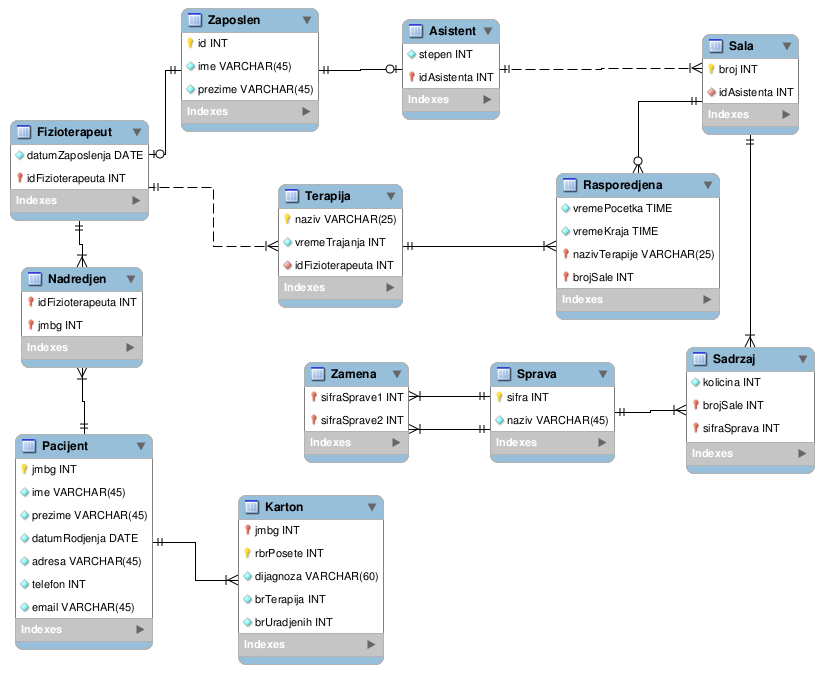
\includegraphics[width=15cm,height=15cm,keepaspectratio]{EER.png}
	\caption{Fizioterapeutska ordinacija}
	\label{fig:dijagram}
\end{figure}

\end{document} 

\end{document}
